% Technical communication from frozen evidence. No new experiments for this note.
\documentclass[letterpaper,10pt]{article}
\usepackage[T1]{fontenc}
\usepackage{lmodern,microtype}
\usepackage[letterpaper,left=.72in,right=.72in,top=.62in,bottom=.62in]{geometry}
\usepackage{amsmath,amssymb,graphicx,booktabs,tikz,enumitem,titlesec,caption}
\usepackage[hidelinks]{hyperref}
\input{glyphtounicode}
\pdfgentounicode=1
\makeatletter
\renewcommand\normalsize{\@setfontsize\normalsize{10.5}{12.5}}
\makeatother
\normalsize
\setlength{\parindent}{0pt}
\setlength{\parskip}{3.5pt}
\setlength{\abovedisplayskip}{5pt}
\setlength{\belowdisplayskip}{5pt}
\setlength{\textfloatsep}{7pt}
\titleformat{\section}{\fontsize{11.5}{13}\selectfont\bfseries}{}{0pt}{}
\titlespacing*{\section}{0pt}{7pt}{2.8pt}
\captionsetup{font=small,labelfont=bf,skip=4pt}
\setlist[itemize]{leftmargin=13pt,itemsep=1pt,topsep=2pt,parsep=0pt}
\hypersetup{pdfauthor={Zhijing Wu},pdftitle={From Failure Discovery to Action Evaluation: A Controlled StressDream Research Investigation},pdfsubject={Independent research preparation; measured scope and proposed follow-up}}
\begin{document}
\begin{center}
{\fontsize{16.5}{19}\selectfont\bfseries From Failure Discovery to Action Evaluation:\\
A Controlled StressDream Research Investigation}\\[5pt]
Zhijing Wu\quad$\cdot$\quad Sichuan University\\[1pt]
Independent technical investigation; unpublished\quad$\cdot$\quad 22 October 2026
\end{center}
\vspace{-5pt}

\section*{1. Research question and motivation}
\textbf{When does failure-oriented world-model steering provide reliable action-level evaluation?}
Does better possible-failure discovery improve true-dynamics action ordering and regret at fixed actions and total compute? The completed oracle, design checks and compatibility/readout pilot do \emph{not} establish that relationship or a new planning algorithm.

\section*{2. Relation to StressDream}
\textbf{Paper-reported evidence.} StressDream optimizes diffusion noise to expose high-impact, plausible futures in frozen action-conditioned world models [1]. It already includes ground-truth Dubins failure checking, plausibility regularization/ablations, candidate-action examples and policy improvement. The present question concerns measurement within that established agenda, not an absence of decision evaluation.

\textbf{Source observations.} Revision \texttt{b16fa067d3d9} [2] raises flip-probability, deterministic-demo, momentum, regularizer and score/noise/sample-alignment questions. Their impact on learned-model performance is unmeasured. The steered ranking comparison remains proposed (Figure~\ref{fig:pipeline}).

\begin{figure}[h!]
\centering
\resizebox{\linewidth}{!}{% Original experimental-contract schematic, not a model-architecture claim.
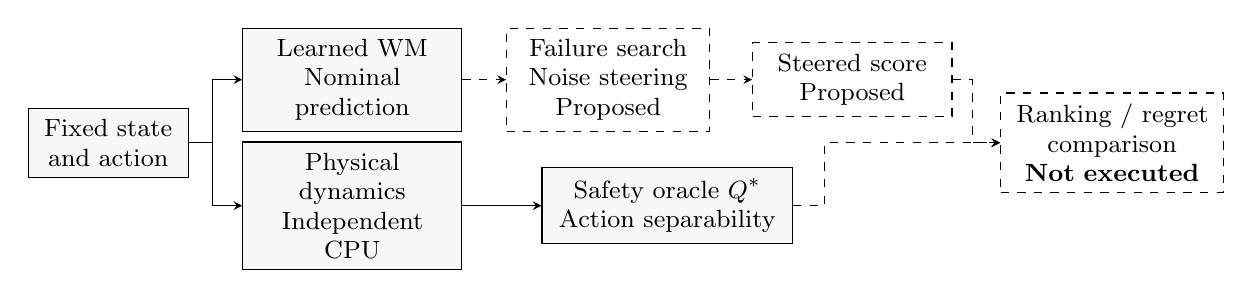
\begin{tikzpicture}[x=1cm,y=1cm,>=stealth,
 box/.style={draw,thin,align=center,inner sep=4pt,minimum height=.85cm,font=\fontsize{9.3}{10.6}\selectfont},
 done/.style={box,fill=black!3},
 proposed/.style={box,dashed,fill=white}]
\node[done,text width=1.75cm] (input) at (.9,.75) {Fixed state\\and action};
\node[done,text width=2.5cm] (wm) at (4,1.55) {Learned WM\\Nominal prediction};
\node[proposed,text width=2.3cm] (steer) at (7.25,1.55) {Failure search\\Noise steering\\Proposed};
\node[proposed,text width=2.25cm] (score) at (10.35,1.55) {Steered score\\Proposed};
\node[done,text width=2.5cm] (physics) at (4,-.05) {Physical dynamics\\Independent CPU};
\node[done,text width=2.9cm] (oracle) at (8,-.05) {Safety oracle $Q^*$\\Action separability};
\node[proposed,text width=2.55cm] (compare) at (13.65,.75) {Ranking / regret\\comparison\\\textbf{Not executed}};
\draw[->] (input.east) -- ++(.3,0) |- (wm.west);
\draw[->] (input.east) -- ++(.3,0) |- (physics.west);
\draw[->,dashed] (wm) -- (steer);
\draw[->,dashed] (steer) -- (score);
\draw[->,dashed] (score.east) -- ++(.25,0) |- (compare.west);
\draw[->] (physics) -- (oracle);
\draw[->,dashed] (oracle.east) -- ++(.4,0) |- (compare.west);
\end{tikzpicture}
}
\caption{Solid: completed oracle or nominal interface work. Dashed: proposed steering and action-ranking comparison. The schematic separates experimental contracts; it does not depict network architecture.}
\label{fig:pipeline}
\end{figure}

\section*{3. Independent finite-horizon dynamics oracle}
The float64 reference implements the released discrete stochastic Dubins dynamics:
\begin{equation*}
\mathbf p_{t+1}=\mathbf p_t+v\Delta t(\cos\theta_t,\sin\theta_t),\qquad
\theta_{t+1}=\theta_t+\Delta t\,\delta_t a_t.
\end{equation*}
Here $v=1\,\mathrm{m/s}$, $\Delta t=.05\,\mathrm{s}$, $|a_t|\le1.25\,\mathrm{rad/s}$ and independent $\delta_t\in\{-1,+1\}$. Position uses the \emph{old} heading. At $H=12$, all $2^{12}=4{,}096$ sign strings are enumerated per query, including safety at $t=0$:
\begin{equation*}
C(s)=x^2+y^2-.25^2,\qquad
Q^*(s,a)=\min_{\delta}\min_{0\le t\le12}C(s_t),\qquad
R(s,\hat a)=\max_a Q^*(s,a)-Q^*(s,\hat a).
\end{equation*}
Larger $Q^*$ is safer; failure is $C\le0$; the released danger head uses $m=-C$.
Sixteen unit tests passed, including scalar checks, signs, update order and witnesses [3]. ``Exact'' means exhaustive \emph{discrete} support in floating point, not certified real arithmetic or continuous-time safety.

\section*{4. Gate 0: separation with weak decision diversity}
All 16 states and five actions remain frozen. At $0.005\,\mathrm{m}^2$, \textbf{12/16 states} are informative and \textbf{106/160 pairs} distinguishable. Yet constant straight-line A0 is practically optimal: maximum robust regret is approximately $0.000176\,\mathrm{m}^2$. The pool supports ranking diagnostics but weakly tests state-dependent choices. This is an oracle design finding, not evidence about StressDream reliability.

\newpage
\section*{5. Gate 0B: a separately declared task extension}
A separate design pool fixed an unfiltered 64-context held-out test with multi-side states and signed controls. Gate 0B \textbf{changes the objective}: expected squared-distance progress toward $(1,0)$ at flip probability $.2$, subject to support safety $Q^*>0$ [3]. At $0.005\,\mathrm{m}^2$, 43 contexts are informative; 41 have meaningfully unique optima, spanning all five IDs. Best-constant mean \emph{task} regret is $0.103087\,\mathrm{m}^2$ (unsafe score: $-4\,\mathrm{m}^2$); all 21 no-safe-candidate contexts remain included. This extension is not StressDream's original objective; its regret scale is not directly comparable with Gate 0.

\section*{6. Gate 1A: compatibility and independent readout}
Both official checkpoints passed size/hash checks, restricted CPU loading and architecture compatibility; prediction-head weights were present [4]. The nominal CPU pilot completed 43 future predictions, 32 paired VAE reconstructions and 215 denoiser forwards in approximately 38.0 model-process seconds, with $0.318\,\mathrm{GiB}$ sampled aggregate peak RAM. These are not steering/full-benchmark costs.

A pixel-only reader, frozen after separate tuning, parsed 16/16 validation images in each paired domain. Position p95 errors were 13.92 mm clean and 13.97 mm reconstructed. The reader is not yet accurate enough for the proposed ranking comparison (Figure~\ref{fig:readout}). For position error bounded by $e$, $|\widehat C-C|\le2\|\widehat{\mathbf p}\|e+e^2$.

\begin{figure}[h!]
\centering
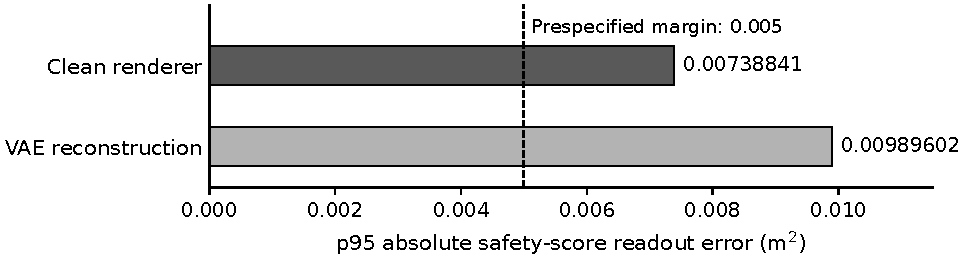
\includegraphics[width=.88\linewidth]{figures/readout_error.pdf}
\caption{Readout p95 on 16 paired validation states: clean $0.00738841$, VAE $0.00989602\,\mathrm{m}^2$. Dashed: prespecified ranking margin $0.005\,\mathrm{m}^2$; per-action readout uncertainty target: $0.00125\,\mathrm{m}^2$. No population interval or world-model failure claim.}
\label{fig:readout}
\end{figure}

\section*{7. Evidence boundaries}
Compatibility \textbf{passes}; Gate 0 ranking remains \textbf{conditional}; Gate 0B expected progress is \textbf{no-go at present}. Both nominal $H=12$ paths missed a coarse consistency tolerance, with model/readout errors confounded. Training flip probability is undocumented (paper $.2$, generator $.4$): common support does not imply equal nominal expectations, and steered sample fractions cannot estimate them.

No steering, full ranking or policy-improvement experiment ran. A final export error lost some tensor/range and future-head logs; retained evidence was recovered without inference replay. No ranking degradation, world-model failure or new algorithmic contribution is established.

\section*{8. Proposed next experimental step --- not executed}
First validate geometry below the frozen score margins. A separately approved nominal/Best-of-$N$/steering comparison would fix states/actions, align noise/latent/score records and match \emph{total} per-action cost (backward passes, regularization, decoding, rescoring). Report supported-failure recall separately from tie-aware ranking/regret. Expected progress also needs probability calibration.

\section*{9. References and reproducibility}
\begingroup\fontsize{9.2}{10.5}\selectfont\setlength{\parskip}{1pt}
\noindent[1] J. Seo et al. \emph{StressDream: Steering Video World Models for Robust Policy Evaluation and Improvement}. CoRL 2026; \href{https://arxiv.org/abs/2606.00267v2}{arXiv:2606.00267v2}.\par
\noindent[2] CMU Intent Lab. \href{https://github.com/CMU-IntentLab/StressDream/tree/b16fa067d3d949ef09ad48a984c62ea8ecbbfe6d}{StressDream source}, revision \texttt{b16fa067d3d949ef09ad48a984c62ea8ecbbfe6d}.\par
\noindent[3] Z. Wu. \href{https://github.com/ZhijingWu/StressDream-Decision-Reliability-Audit/tree/main/experiments}{\emph{Dubins Oracle and Decision-Diversity Audits}} (Gate 0/0B), 2026. Unpublished audit records.\par
\noindent[4] Z. Wu. \href{https://github.com/ZhijingWu/StressDream-Decision-Reliability-Audit/tree/main/experiments/gate1a}{\emph{Checkpoint/Readout Compatibility Pilot}} (Gate 1A), 2026. Unpublished audit records.\par
Public reproducibility: \url{https://github.com/ZhijingWu/StressDream-Decision-Reliability-Audit}. Frozen configurations, commands, numerical evidence and SHA-256 mappings are public; selected reports are sanitized copies. This note adds no experiments or complete paper reproduction.
\endgroup
\end{document}
